\subsection{分式环的整闭包}

设 A 是环，R 是 A-代数，S 是 A 的乘性子集。回忆（第 II 章，§ 2，第 8 节），\(\mathbf{S}^{-1}\mathbf{R}\) 具有典范的 \(\mathbf{S}^{-1}\mathbf{A}\) -代数结构。

命题 16. 设 A 是环，R 是 A-代数，A' 是 A 在 R 中的整闭包，S 是 A 的乘性子集。则 \(\mathbf{S}^{-1}\mathbf{A}\) 在 \(\mathbf{S}^{-1}\mathbf{R}\) 中的整闭包是 \(\mathbf{S}^{-1}\mathbf{A}'\) 。

设 \(b / s\) 是 \(S^{-1}A'\) 的元素（ \(s \in S, b \in A'\) ）。由于图

\pandocbounded{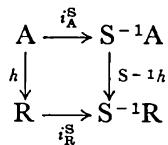
\includegraphics[keepaspectratio]{images/part002_55e4c379.jpg}}

是交换的，\(b / 1\) 在 \(S^{-1}A\) 上是整的（第 1 节，命题 2）。由于 \(1 / s \in S^{-1}A\) ，故 \(b / s = (b / 1)(1 / s)\) 在 \(S^{-1}A\) 上是整的。

反之，设 \(r / t\)（ \(r \in \mathbb{R}\) ，\(t \in \mathbb{S}\) ）是 \(\mathbf{S}^{-1}\mathbf{R}\) 中在 \(\mathbf{S}^{-1}\mathbf{A}\) 上整的元素；则 \(r / 1 = (t / 1)(r / t)\) 在 \(\mathbf{S}^{-1}\mathbf{A}\) 上是整的。于是存在形如

\[
(r / 1) ^ {n} + (a _ {1} / s) (r / 1) ^ {n - 1} + \dots + (a _ {n} / s) = 0,
\]

的关系式，其中 \(a_{i} \in \mathbf{A}\)（ \(1 \leqslant i \leqslant n\) ），\(s \in \mathbf{S}\) 。这个关系式也可以写成

\[
(s r ^ {n} + a _ {1} r ^ {n - 1} + \dots + a _ {n}) / s = 0
\]

从而存在 \(s' \in S\) 使得 \(s'^{n}(sr^{n} + a_{1}r^{n-1} + \cdots + a_{n}) = 0\) ；由此推出 \((s'sr)^{n} + s'a_{1}(s'sr)^{n-1} + \cdots + s'^{n}s^{n-1}a_{n} = 0\) 。因此按定义有 \(s'sr \in A'\) ，从而 \(r/1 \in S^{-1}A'\) ，且 \(r/t \in S^{-1}A'\) 。

推论 1. 设 A 是整环，A' 是它的整闭包，S 是 A 的乘性子集且 \(0 \notin S\) 。则 \(S^{-1}A\) 的整闭包是 \(S^{-1}A'\) 。

A 的分式域 R 也是 \(S^{-1}A\) 的分式域，因为 \(0 \notin S\) （第 II 章，§ 1，第 1 节，注 7）；对 R 应用命题 16 即得。

推论 2. 设 A 是整环，K 是它的分式域，R 是 K 上的代数，B 是 A 在 R 中的整闭包。R 中在 K 上代数的元素（第 1 节，例 1）恰是形如 \(a^{-1}b\) 的元素，其中 \(b \in \mathbf{B}\)，\(a \in \mathbf{A}\)，\(a \neq 0\) ；若 L 是 K 在 R 中的代数闭包，则存在包含在 B 中的 L 在 K 上的基。

第一个断言由命题 16 应用于 \(\mathbf{S} = \mathbf{A} - \{0\}\) 的情形而得。若 \((x_{i})_{i\in I}\) 是 \(\mathbf{L}\) 在 \(\mathbf{K}\) 上的一组基，则对每个 \(i\in I\) 存在元素 \(a_{i}\neq 0\) 属于 \(\mathbf{A}\) ，使得 \(a_{i}x_{i}\in \mathbf{B}\) ；于是 \((a_{i}x_{i})_{i\in I}\) 也是 \(\mathbf{L}\) 在 \(\mathbf{K}\) 上的基。

推论 3. 设 A 是整环，\(\Omega\) 是 A 的极大理想组成的集。为使 A 是整闭的，必须而且只需对所有 \(\mathfrak{m} \in \Omega\) ，\(\mathbf{A}_{\mathfrak{m}}\) 都是整闭的。

由推论 1 可知该条件是必要的。该条件也是充分的，因为 \(\mathbf{A} = \bigcap_{m \in \Omega} \mathbf{A}_m\)（第 II 章，§3，第 3 节，公式 (2)），故只需应用第 2 节命题 8 的推论即可。

推论 4. 设 A 是整环，K 是它的分式域，S 是 A 的乘性子集且 \(0 \notin S\) 。

\begin{enumerate}
\def\labelenumi{(\roman{enumi})}
\item
  设 B 是 K 的子环且在 A 上是整的，f 是 A-模 B/A 的零化子。则 \(S^{-1}f\) 包含在 \((S^{-1}A)\) -模 \(S^{-1}B/S^{-1}A\) 的零化子之中，且当 B 是有限生成 A-模时等于这个零化子。
\item
  设 A' 是 A 的整闭包。为使 \(S^{-1}A\) 整闭，只需 A-模 A'/A 的零化子 f 与 S 相交。若 A' 是有限生成 A-模，这个条件也是必要的。
\setcounter{enumi}{0}
\item
  由于 \(\mathfrak{f}\mathbf{B} \subset \mathbf{A}\) ，有 \((\mathrm{S}^{-1}\mathfrak{f})(\mathrm{S}^{-1}\mathbf{B}) \subset \mathrm{S}^{-1}\mathbf{A}\) ，因而 \(\mathrm{S}^{-1}\mathfrak{f}\) 包含在 Ann \((\mathrm{S}^{-1}\mathrm{B} / \mathrm{S}^{-1}\mathrm{A})\) 之中。若 \(\mathbf{B}\) 是有限生成 A-模，则等式 \(\mathrm{S}^{-1}\mathfrak{f} = \operatorname{Ann}(\mathrm{S}^{-1}\mathrm{B} / \mathrm{S}^{-1}\mathrm{A})\) 是第 II 章 § 2 第 4 节公式 (9) 的特殊情形，这里 \(\mathrm{S}^{-1}\mathrm{B} / \mathrm{S}^{-1}\mathrm{A}\) 典范地等同于 \(\mathrm{S}^{-1}(\mathrm{B} / \mathrm{A})\) 。
\item
  由推论 1，\(\mathbf{S}^{-1}\mathbf{A}'\) 是 \(\mathbf{S}^{-1}\mathbf{A}\) 的整闭包。由于关系 \(\mathfrak{f} \cap \mathbf{S} \neq \varnothing\) 与 \(\mathbf{S}^{-1}\mathfrak{f} = \mathbf{S}^{-1}\mathbf{A}\) 等价（第 II 章，§ 2，第 5 节，注），(ii) 是 (i) 的直接推论。
\end{enumerate}

若 B 是 K 的子环且在 A 上是整的，则 B/A 的零化子 f（按定义等于传递子 A: B（第 I 章，§ 2，第 10 节））有时称为 B 在 A 中的导子。

推论 5. 设 A 是整环，A' 是它的整闭包，f 是 A-模 A'/A 的零化子。假设 A' 是有限生成 A-模。则使 A \(_{p}\) 不是整闭的 A 的素理想 p 恰是包含 f 的那些素理想。

这由推论 4 (ii) 应用于 S = A - p 立即得出。

注意，在推论 5 的假设之下 f ≠ 0，因为 A' 是有限生成 A-模，且 K/A（K 是 A 的分式域）的每个元素的零化子都 ≠ 0。

* 在代数几何中，推论 5 与上面的注表明：仿射簇 V 的非正规点组成一个异于 V 的闭集。*

